\documentclass{acm_proc_article-sp}
\usepackage{graphicx}
\usepackage{mathtools}
\usepackage[utf8x]{inputenc}
\usepackage{parskip}

\setlength{\parindent}{0pt}
\setlength{\parskip}{\baselineskip}

\begin{document}

\title{Access Control Policy Verification and Repairing in Alloy}

\numberofauthors{1}

\author{
\alignauthor Alexandr Murashkin, Matthew Ma \\
       \affaddr{The David R. Cheriton School of Computer Science}\\
       \affaddr{University of Waterloo}\\
       \affaddr{Waterloo, ON, Canada}\\
       \email{m22ma, amurashk@uwaterloo.ca}
}
\date{2 December 2012}
\maketitle

\begin{abstract}
In product line development, there is a problem of discovering product configurations that are optimal with respect to set of objectives within a product family. There are tools that solve the problem, but in most cases there are multiple optimal product configurations, and there is room for innovation here regarding visualization, choosing a subset of optimal products, trade-off analysis and comparison of generated configurations. We propose a software tool - a GUI that visualizes the set of optimal products and offers certain visualization and human interaction techniques to accomplish these tasks. Our pilot evaluation of this tool has shown feasibility of the approach and given some directions of further research in this area.  
\end{abstract}


\category{H.5.2}{Information Interfaces and Presentation}{User Interfaces}[Graphical user interfaces (GUI)]

\terms{Product lines, Multi-objective optimization, Pareto front, visualization}

\keywords{Visualization, GUI, bubble chart, user experiment} % NOT required for Proceedings

\section{Introduction}




\section{Related work}

Regarding access control policy verification, there are several various related approaches.
\cite{Hughes:2008:AVA:1459278.1459282} proposes encoding XACML access control policies  ordering relations and then translation of them into SAT solver for verification. \cite{4258517} describes inconsistency checking in role-based access control policies (RBAC).  \cite{Fisler:2005:VCA:1062455.1062502} proposes Margrave - a great tool for access control policies (XACML and other formats) verification and change-impact analysis. \cite{Jackson:2000:AFR:357474.355063} proposes Alloy Analyzer as first-order logic verification tool (there is a corresponding book \cite{jackson:alloy}).

For Access control policy verification in Alloy: 
1) http://www.cs.ucsb.edu/~bultan/publications/tech-report04.pdf
2 - WE USE IT!! ) http://w3.uqo.ca/notere05/documents/logrippo.pdf, need a citation.

Regarding repairing XACML access control policies, it does not seem to be a lot of prior related work. Rather than that, \cite{Zhang:2004:SVA:1029133.1029141} offers access control policies verification in the language called RW and then synthesize verified specifications in XACML. \cite{Bravo:2007:RIX:1783534.1783545} considers another type of access control policies - XML write access control policies - offers repairs in case of that some actions can be simulated by multiple another actions. 

Regarding model repairing in general, \cite{Xiong:2009:SAM:1595696.1595757} proposed .... for i don't know what, need to read :) . \cite{Reder:2012:CRT:2351676.2351707} proposes repair trees for inconsistency solving in design models.

The proposed technique of repairing inconsistencies - sketching - was described in the thesis http://people.csail.mit.edu/asolar/papers/thesis.pdf .

Need to look at this - probably needed - http://people.csail.mit.edu/eskang/talks/mit-security-seminar-nov2012.pdf .

The specification of XACML:
http://docs.oasis-open.org/xacml/2.0/access_control-xacml-2.0-core-spec-os.pdf


\subsection{Background}

The problem occurs in product line development. Product line engineers, model architects, or developers design a product family - set of different products with shared architecture and common components \cite{ClementsNorthrop2001}. Individual products are characterized by selection of features from the feature model of the product family \cite{Kang90}. Some features contain quality attributes that impact on the product total quality attributes - so called extra-functional features \cite{Benavides05automatedreasoning}. For example, presence of second CPU on mobile device makes the phone total performance rate two times higher, but increases the phone total cost. The challenge faced by engineers is discovering which products are optimal with respect to a set of goals (e.g. to achieve maximal performance) \cite{474}.

There is a tool named Clafer Multi-Objective Optimizer (ClaferMoo) \cite{474}. The tool takes a feature model with quality attributes and set of objectives (written with a lightweight modeling language called Clafer \cite {bak:claferfeature}) as input), solves multi-objective optimization problem with respect of the objectives and generates all optimal model configurations. In case of product lines, the feature model defines a product family, and the optimal model configurations are simply optimal product configurations, or prospective products.

\begin{figure*}[ht]
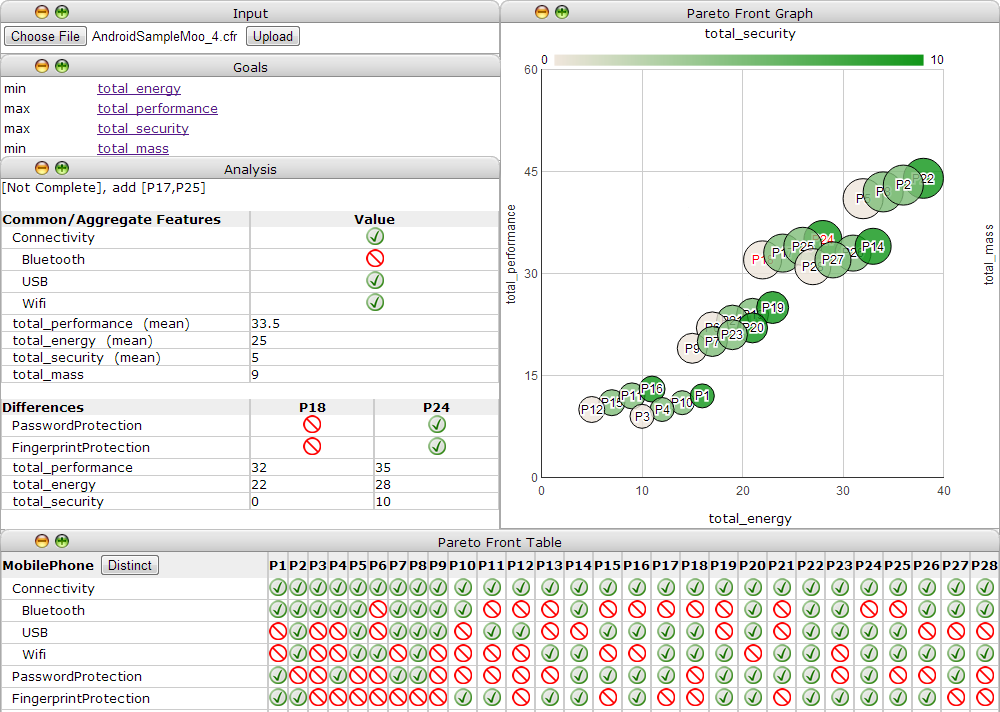
\includegraphics[width=\textwidth]{gui.png}
\caption{ClaferMoo Visualizer: user interface}    
  \label{fig:gui}
\end{figure*}


\subsection{Motivation}

The existing ClaferMoo tool was not designed to provide a good user interface. The tool outputs generated configurations one-by-one as a structured text. The problem is that product families can contain lots of features, and multiple optimal  configurations can be generated. If manufacturer needs to choose 5 final products out of 50 possible configurations, then the task becomes difficult: manual comparison of generated product configurations is, obviously, time and effort consuming. Moreover, there are trade-offs between several features (e.g. performance versus cost) that cannot be processed in an automatic way, so trade-offs related tasks have to be completed by human in an effective and straight-forward way.

\subsection{Problem statement}

Currently there is lack of commonly used techniques and tool support that help manufacturers effectively manage generated product configurations, compare them side-by-side, understand trade-offs, and pick up the most suitable products for manufacturing. Current visualization solutions do not allow interactive exploration and often are not connected to design decisions. The objectives are to build an an effective and usable software tool that can visualize the product models, trade-offs and help to identify an optimal solution. The tool also has to be light-weight and cross-platform and has to use ClaferMoo as a back-end.

\subsection{Related terms and conventions}

The paper does not deal with multi-objective optimization problem directly, so there is no problem description in this paper. The only related term used - \textit{Pareto front} - is a set of non-dominant solutions of multi-objective optimization problem. In this paper, Pareto front is just a set of optimal product configurations generated by ClaferMoo tool. For instance, for some product family model of mobile phones, ClaferMoo generates several product configurations: mobile phone $P1$, mobile phone $P2$, mobile phone $P3$, and mobile phone $P4$ that have the highest total performance and the lowest total mass. Each phone can have distinct features (e.g. $P1$ and $P4$ have second CPU, $P1$ and $P3$ have physical keyboard) and total quality attributes (e.g. total performance of $P1$ is 500 MHz and total mass of $P4$ is 300 grammes). Pareto front is simply the set $P = \{P1, P2, P3, P4\}$. In this paper, the terms "set of optimal product configurations", "set of optimal products", "Pareto front" are used as synonyms and often denoted as just "products". 

\subsection{Paper structure}

Implementation section gives brief overview of our solution - a software tool, shows two techniques of visualizing Pareto Front - the graph and the table, and opportunities of the tool related to the Pareto Front analysis. User evaluation section contains results of our pilot study - a controlled experiment aimed to do the initial evaluation of the implemented tool and visualization techniques. Related work section compares the work to related approaches regarding Pareto front visualization and user interfaces.
Conclusion section summarizes completed work and lists work implications.

\section{Implementation}

\subsection{Overview}

We implemented a web-based tool called ClaferMoo Visualizer. The tool is a GUI for ClaferMoo tool and can be considered as a presentation layer, since its input data is actually the output data of ClaferMoo. The user interface is mainly composed of several collapsible windows (Fig. \ref{fig:gui}). Each window has certain purposes as listed below. 
\begin{itemize}
\item Input - allows input file uploading.
\item Goals - shows the multi-objective optimization goals.
\item Pareto Front Table - a tabular representation of Pareto Front.
\item Pareto Front Graph - a graphical representation of Pareto Front.
\item Analysis - shows commonalities and differences among Pareto Front, and class equivalences.
\end{itemize}

A typical workflow is the following. First, user navigates to the tool page, uploads a Clafer file using the input window, and ClaferMoo runs successfully. The tool processes the data transferred from ClaferMoo and fills in the windows Goals, Pareto front table and Graph. Then user can perform various actions depending on use cases. User can inspect the table view and see what products are generated, what features and quality attributes they have. User can inspect the graph and see all the products there displayed as labeled bubbles, view the popup with concrete values for each product, change the dimensions that should be visualized on X and Y axes, and using opacity and bubble size. User can select products on the graph for analysis, the corresponding window is filled in with selected products, and user can see commonalities and differences. User can upload another file or just close the browser page window when finished working.  

\subsection{Pareto Front Table}

\begin{figure}[h]
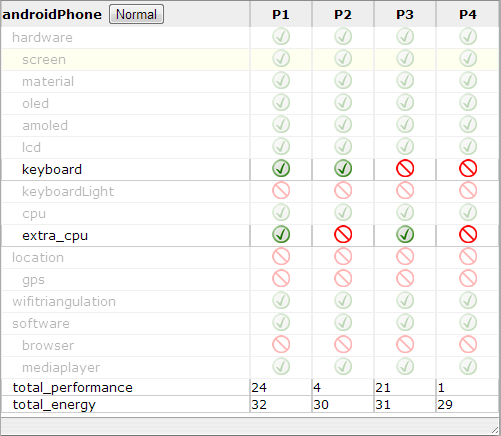
\includegraphics[width=0.5\textwidth]{table.png}
\caption{Pareto Front Table. Distinct features are highlighted}    
  \label{fig:table}
\end{figure}

Pareto Front Table (Fig.\ref{fig:table}) is a straight-forward way to represent the whole set of product configurations. Row headers represent features and total quality attributes, the hierarchical structure is preserved. Column headers represent product configurations and denoted as $P1, P2, ... PN$, $N$ - the number of generated configurations. Cells at the intersection of column $C$ and row $R$ are defined in the following way:
\begin{itemize}
\item If $R$ is a feature, and product $C$ has the feature, then the cell contains "yes" (a green tick), otherwise "no" (a red crossed circle).
\item If $R$ is a quality attribute, then the cell contains the numeric value of the quality attribute.
\end{itemize}

\subsection{Pareto Front Graph}

Pareto Front Graph is aimed to graphically represent Pareto Front in such a way that user can clearly see the whole set of solutions and pick one or more solutions for the analysis. The graph is actually a bubble chart  (Fig.\ref{fig:graph}).

Let $m$ denote the cardinality of the metric space, and $s$ the cardinality of the solution space. Let's denote bubble chart representations as $X$ (horizontal axis), $Y$ (vertical axis), $Z$ (bubble opacity) and $T$ (bubble size). 
Bubble chart appears to be good for representing a Pareto Front with $m$ is less than or equal to 4, and $s$ is not very big (the upper bound depends on diversity of configurations and available space on the screen). Moreover, there are some special cases:

\begin{itemize}
\item If $m = 2$, then $X$ and $Y$ representations are used.
\item If $m = 3$, then $X$, $Y$ and $Z$ representations are used.
\item If $m = 4$, then $X$, $Y$, $Z$ and $T$ representations are used. 
\item If $m > 4$, then the user may choose which metrics are to be represented using $X$, $Y$, $Z$ and $T$ representations by drag-and-drop from the "Goals" window onto the four sides of the graph. So projections are used to deal with higher dimensions. 
\end{itemize}

In Fig.\ref{fig:graph} showing the graph of the phone example, $X$ axis represents total energy consumption. Bubbles to the right represent products with higher energy consumption, to the left - lower consumption. $Y$ coordinate - total performance. The higher the items, the more performance they can provide. $Z$ representation - total security. The more opaque bubble, the more security the corresponding product has. $T$ (bubble size) represents total mass. Wider bubbles correspond to heavier phones. So, all bubbles are presented according to their total energy and total security ($X$ and $Y$ values), their opacity ($Z$ representation) is proportional to total security, and size ($T$ representation) is proportional to total mass (Fig.\ref{fig:graph}).

Some representations can be assigned in a way that analogies can help users with the future analysis. Representation $T$ (bubble size) can denote something like mass, volume or size: "heavier" items will be bigger, "lighter" - smaller. Representation $Z$ (bubble opacity) can denote something that has the notion of "good", "bad" and "intermediate" : security, pressure, etc.: fully transparent means completely insecure, fully opaque means "totally secure".

Users can mouse over on some bubble, and the popup appears that shows the exact quality attribute values. Users can also pick one or more products for analysis by clicking on the corresponding bubbles on the graph.

\begin{figure}[h]
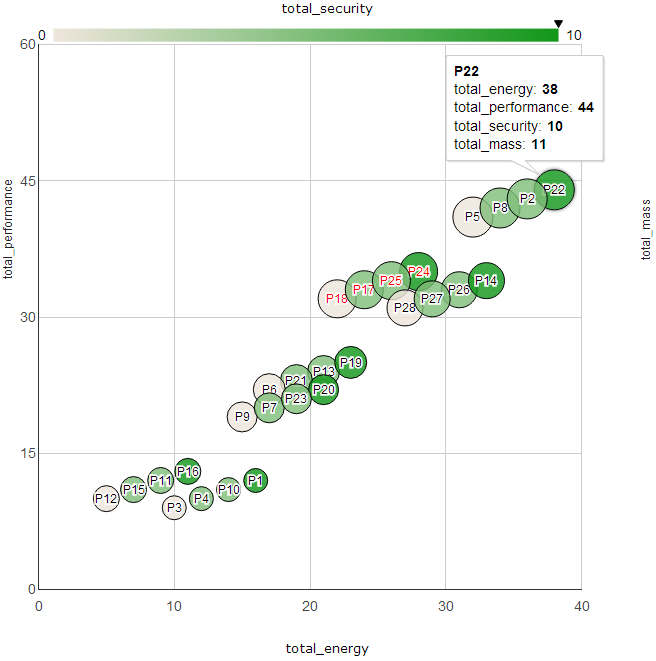
\includegraphics[width=0.5\textwidth]{graph.png}
\caption{Pareto Front Graph for the mobile phone example. Legends: horizontal axis -  total energy, vertical axis - total performance, bubble opacity - total security (label and legend are shown at the top),  bubble size - total mass (label shown at the right). Popup window shows exact values of the product in all 4 dimensions.}    
  \label{fig:graph}
\end{figure}

\subsection{Pareto front analysis}

The Analysis window is designed to support the following tasks:
\begin{itemize}
\item Show features of one selected product.
\item Show common features of multiple selected products.
\item Show differences among multiple selected products.
\item Denote whether common features of the selected products define a "complete equivalence class".
\item Denote what products can be added to the selection set to define a "complete equivalence class".
\end{itemize}

The \textit{complete equivalence class} notion is a largest set of products which have the same commonality - set of pairs $(f, v)$, where $f$ - a feature from product family, $v$ - a boolean that denotes whether this feature included in certain product. Adding another product to the set will decrease the commonality. Formally, we can define a relation $R$ over Pareto front $P$, $aRb$ if and only if the products $a$ and $b$ have the same commonality $C$.

Considering the phone example, if user picks P18 and P24, then Analysis window displays that the only different features are $PasswordProtection$ and $FingerprintProtection$: P18 has neither, P24 has both. The features $Connectivity$ (a composite feature), $USB$ and $WiFi$ are present in both products, as well as both have the same total mass. $Bluetooth$ is not included in either. So P18 and P24 have the same commonality set \{ (Connectivity, $true$), (USB, $true$), (WiFi, $true$), (Bluetooth, $false$) \} (Fig.\ref{fig:analysispartial}). Mean value (if quality attribute value is not the same among all selected products) and exact value (if quality attribute value is the same among all selected products) of quality attributes are shown in the Common/Aggregate features region.

\begin{figure}[h]
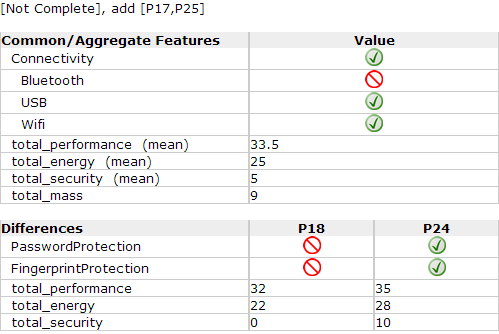
\includegraphics[width=0.5\textwidth]{analysispartial.png}
\caption{Analysis window: P18 and P24 are picked up}    
  \label{fig:analysispartial}
\end{figure}

Now, to make the equivalence class complete, the tool recommends to add P17 and P25: if the user picks them, then a complete equivalence class is defined: the set of all products with $USB$ and $WiFi$ and $not$ $Bluetooth$ (Fig.\ref{fig:analysisfull}). 

\begin{figure}[h]
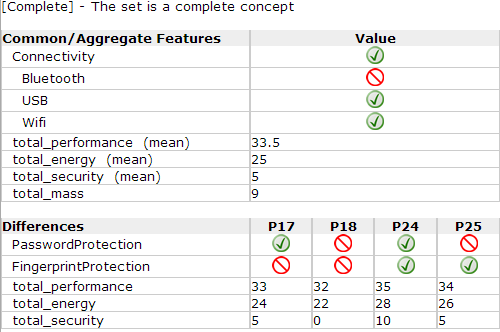
\includegraphics[width=0.5\textwidth]{analysisfull.png}
\caption{Analysis window: a complete equivalence class is shown}    
  \label{fig:analysisfull}
\end{figure}

Actually complete equivalence classes might be visualized as separate clusters (See evaluation and future work section for ideas of clustering).

\section{Evaluation}

\subsection{Form and purpose}

The aim of the user evaluation was to determine whether visualization and interaction techniques implemented in the tool are good enough for now, and what is the further direction of development. This evaluation is a pilot study, not the final one: we are planning to conduct further evaluations with our industry partners.

To evaluate our tool, we performed a controlled experiment in which the participants were asked to perform a predefined set of tasks using the tool and answer provided questions. Occasionally, we also asked additional questions as appropriate in the given context.

The experiment included 11 tasks split into 3 groups based on the difficulty level followed by a final questionnaire (Appendix \ref{A}). Difficulty levels made the main part of the experiment well-structured and reduced learning effect. The final questionnaire was used to get an informal feedback upon the tasks completion. Three subjects - two full-time graduate students and one postdoctoral fellow of Generative Software Development Lab, University of Waterloo. All three subjects have background in product lines development and two subjects have expertise in multi-objective optimization, so no background questionnaire was used to determine their background. Prior to the experiment, we gave a short presentation of tool features to the participants, intended ways of using the tool, and completion of some sample tasks.

\subsection{Results}

\subsubsection{Task completion}

All participants were able to complete almost all tasks: some tasks were not understood properly or brought confusion (for example, the question in T10 did not clarify that common features are asked, not common quality attributes as one subject understood), but after clarification (the experiment form allowed that), the subjects were able to complete them. Two subjects completed question 1 in T11 in the way they were not supposed to do: they did not notice the suggestion of the tool and manually looked at the Pareto front table and searched for the products that have USB and Bluetooth. However, the result was still correct.

Not all tasks required subject to provide some concrete correct end result. For instance, for question 3 in the task T11, all subjects made conclusions that total mass differs not significantly, but one of them made a notice that the domain knowledge is important to determine whether the difference in total mass significant or not.

\subsubsection{Pareto front visualization}

Regarding the visualization, all three participants found the bubble chart visualization useful. Participants were able to make decisions in 4-dimensional space, compare bubbles and pick up the ones they needed.

Regarding limitations, all participants noticed that is is hard or even impossible to compare products that differ in third and forth dimensions by a small value. If products differ in positions ($X$ and $Y$ axises), it is easy to notice, because one pixel difference on the plane is noticeable. In contrast, regarding $Z$ and $T$ dimensions this exact comparison seems to be not possible in bubble charts. The experiment has shown that the bubbles of products with $total\_mass = 2$ and $total\_mass = 3$ appeared to have almost the same size, and it was hard to notice a small change in diameter. In the example, total security had three discrete values: $0$, $5$ and $10$. Two participants quickly understood the difference among all the three opacities, but one was confused with zero value: he said that from the graph it is not clear whether the product represented by the bubble has exact zero total security or slightly bigger. Probably, the reason was that bubbles representing products with 0 total security actually were not 100\% transparent: they were slightly grayed (internal bubble chart feature for bubble readability improvement).  Fortunately, all three participants could rely on the popup feature of the graph to know the exact values of quality attributes. The idea to deal with the limitation in the future is the following: the user chooses all the bubbles that look to be the same, there should be an option to zoom in, or to take them all out and display on a separate graph. The scale is recalculated in order to make the differences more noticeable. Another limitation noticed by one participant is that bubble diameter matters, and this can limit the opportunities of such a visualization (lack of the space on the screen). Noticed limitations is a good result.

There were some small problems that included the lack of conventions how the labels of $Z$ and $T$ representations should be specified and where should they be located. Current position of labels was misleading for one participant: he said that the mass label ($T$ representation) should be put in another place, otherwise it is confused with meaning of $Y$ axis. Moreover, as two participants mentioned, the mass label should be more informative. Probably, the label should include few empty bubbles with distinct sizes to show that total mass is proportional to the bubble size.
Two participants noticed the correlation between mass, security and performance, but they were not asked to do so. It is a good indicator that users can reason among multiple dimensions with this visualization.
Overall, Pareto front visualization using bubble charts seems to be very promising and natural to use.

\subsubsection{Clustering}

It is interesting that during our experiment all three participants started to talk about clustering before they met the question on that. They used various metaphors: "line to separate products", "scope", "square" or "range" to represent the same notion - cluster. It appears that grouping products together by some algorithm (by common features, common values of quality attributes, or proximity) would be helpful for them to complete various tasks or just to compare together two groups. Two participants found the idea of clustering by feature useful, another one said that this would be probably useful, but for some concrete scenarios. One participant noted that he is not sure that equivalence classes is the best way to do clustering. So, clustering appeared to be an important prospective feature.

\subsubsection{Other problems and suggestions}

There were other suggestions and problems related to the tool in general. All three participants mentioned that filtering by features is important, and there is a need in top-down decision making: given a set of features, how to choose suitable products that have these features. Participants wanted to select products in the Pareto front table by clicking on the columns and also by clicking on the features in the table. The tool did not allow to accomplish this, but users mentioned that they would add necessary constraints to the model, so the tool will recalculate Pareto front and give the right result. In any case, this is a good point for the future work. 

Two participants brought some interesting point: in task T8 they could make the conclusion that certain features (PasswordProtection and FingerprintProtection) contribute to total security even without knowledge about the exact values of feature attributes. However, they wanted to look at the original model to give a precise answer. 

There were other minor usability problems. Selection and unselection of bubbles was not clear, since users were not asked to pay attention on dealing with selections properly assuming this is easy. One user experienced problems while finding bubbles with certain label on the graph. Anyway, the problems mentioned in this section are specific to use cases and we can easily resolve them in the future.



\section{Future work}

Important future work includes identifying use cases for the tool from engineers working for our industrial collaborators, implementing support for theses use cases, and conducting evaluation with the engineers. Next, a work in Pareto Front clustering is encouraged, since all the user evaluation subjects mentioned clustering. Instead of representing the whole Pareto Front, users would be able to focus on clusters. Clustering can be based not only on bubble positions, but on the features shared by corresponding products, so each cluster can be defined using a notion of complete equivalence class. It appeared that clustering will be useful for visualization and top-down analysis purposes. And finally, there is an idea to implement top-down analysis. It turned out that current implementation is focused more on bottom-up exploration, given that user sees individual products. However, during the experiment, users wanted to make decisions from top to bottom, filtering out the products automatically by presence or absence of certain features.

\section{Conclusion}

\subsection{Summary}

We implemented a working and usable tool, which can be presented as an effective graphical user interface for ClaferMoo tool. User experiment showed that the implemented tool helps to successfully complete basic tasks and to make conclusions on Pareto fronts in 4-dimensional space as well as revealed future work directions.

\subsection{Implications}

\begin{itemize}
\item Four-dimensional Pareto front visualizations can be effectively implemented using bubble charts.
\item Pareto front analysis can be simplified with usage of effective visualizations.
\item Top-down Pareto front analysis is necessary in some scenarios.
\item Product configuration sets can be characterized by common features of its elements.
\end{itemize}

\bibliography{sigproc-sp}{}
\bibliographystyle{plain}

\appendix
\section{User experiment tasks and questionnaire} \label{A}

\underline{ \textbf{I. Introductory presentation}}

\underline{ \textbf{II. Tasks}}

Tasks are split into 3 categories: \textbf{Overview}, \textbf{Graph} and \textbf{Case Studies}. All tasks are to be performed using the think-aloud protocol, that is, the participants should verbally describe what and why they are doing. All tasks are based on the file \textit{AndroidSampleMoo\_4.cfr}.

\textbf{1. Overview:}

\textbf{T1.} Upload a model file \textit{AndroidSampleMoo\_4.cfr}.\\
\textbf{T2}. Tell what features and quality attributes are specified in the Android phone model.\\
\textbf{T3}. Tell what objectives are presented in the Android phone model.\\
\textbf{T4}. Tell how many Android phone configurations are generated.\\

\textbf{2. Graph:}

\textbf{T5}. Identify 4 phones with the highest total performance (Just say: “P29, P30, P12, P4”, for instance). What is their total mass?\\
\textbf{T6}. Identify a phone with the lowest energy consumption. What is its total performance?\\
\textbf{T7}. Identify the phones with very low total mass.\\
\textbf{T8}. How many phones have perfect (highest) total security? What features contribute to total security?\\

\textbf{3. Cases studies:}

\textbf{T9.} Your boss says that among all the sets of phones you need to issue only one. He says that he needs to choose one among the phones with the best total performance. He is OK with any high energy consumption, since new Android battery is very good. He says he does not need a perfect total security, but it should be more than 0. So he is OK to sacrifice total security to get more total performance.\\
\textit{Your actions:}\\
1) Which product(s) will you choose and why?\\

\textbf{T10.} Your boss says that it is interesting that bubbles representing P5, P8, P2, and P22 are located close to each other. And he wants to know why this happened. Because, maybe, the phones are equivalent in some sense and we can consider them separately as an equivalence class.\\
\textit{Your actions:}\\
1) What do the products have in common and what are the differences?\\
2) Why the bubbles are located close to each other?\\

\textbf{T11.} Your boss needs you to analyze the total performance and total mass of all prospective phones that have USB and WiFi features. He knows that P5, P8, P2, P22 and P18 have USB and WiFi. But he wants to consider all the phones that have USB and WiFi features.\\
\textit{Your actions:}\\
1) Make the set to be a complete equivalence class by adding other relevant products to it.\\
2) Among the selected products within the equivalence class, what is the:\\
	Minimal,\\
	Mean,\\
	Maximal\\
total performance? Are the phones differ in total mass significantly or not?\\
3) Based on the question above, is it reasonable for the boss sacrifice total mass to gain more total performance?\\

\underline{ \textbf{Questionnaire}}\\

\textbf{Q1.} Do you find the idea of representing the products in a four-dimensional space using bubble chart useful? Any comments on that? Are there limitations? Does the representation of the four dimensions make it easy to find “better” products?\\
\textbf{Q2.} What do you think about the notion of the complete equivalence class? What is it and how it can be used? Describe it in your own words.\\
\textbf{Q3.} I noticed that I can group products together based on their features, so each cluster will be denoted by an equivalence class. Let’s call it “clustering by features”. Do you think it is a good idea or not?\\



\balancecolumns
\end{document}
